\chapter{Niet triviale stromingsprofielen}\label{sec:numeriekeMethoden}
Voor niet triviale stromingsprofielen is het niet altijd haalbaar om een volledig analytische oplossing te vinden. Daarom onderzoeken wij nu in het algemeen continue stromingsprofielen met behulp van numerieke methoden.

Het softwarepakket MATLAB is een geschikte omgeving om stelsels differentiaalvergelijkingen, zoals gevonden in sectie \ref{sec:Eliminatie van u}, op te lossen. Een functie als \mcode{ode45} is een voordehandliggende keuze bij het doorrekenen van zo'n stelsel. Voor meer achtergrondinformatie over dit soort functies, zie bijlage \ref{sec:odeSolver}.

Het bleek mogelijk om in het gevonden stelsel differentiaalvergelijkingen \(\lambda_1\) te elimineren en alleen nog afhankelijkheid van \(\lambda_2\) te hebben. Omdat alle relevante vergelijkingen continu zijn stelt dit ons in staat om met behulp van de bisectiemethode te zoeken naar de optimale \(\lambda_2\). Op de bisectiemethode wordt dieper ingegaan in bijlage \ref{sec:bisectiemethode}.

Bij het zoeken naar oplossingen voor specifieke stromingsprofielen blijkt het regelmatig lastig om goede startwaarden te vinden voor schaduwvariabele \(\lambda_2\). Omdat we geen manier hebben mogelijke waardes voor \(\lambda_2\) te vinden waren we vaak aangewezen op het proberen van willekeurige waardes.


Dit wordt ge\"illustreerd in het volgende voorbeeld.

\section{Met een speedboot over de Nijl}
	Een voorbeeld van een toepassing van dit model in het 'alledaags' leven, is het scenario waarin iemand besluit om in de maand juli met een 2015 V22 RF\cite{een speedboot} Speedboot de rivier Nijl over te steken.\\ De Nijl heeft een gemiddelde breedte \(b\) van ongeveer \(2.8~km\)\cite{Nijlbreedte}.
Deze boot heeft een gemiddelde snelheid van \(38~km/h\) of \(0.63~km/min\) als de boot normaal beladen is.\cite{bootstats}
De stroming is sterker in het midden van een rivier dan aan de oevers waar de stroming nagenoeg \(0\) is.
Dit laat zichbeschrijven door een sinuso\"ide:
\begin{align}
	S(x_1) = a \cdot \sin(\frac{\pi }{b}x_1)
\end{align}
Hierbij is \(a\) een stromingsconstante. \\
De eenheid van \(a\) is \(km/min\).
Om \(a\) te bepalen beschouwen we de gemiddelde waterverplaatsing van de Nijl.
De gemiddelde waterverplaatsing \(Q_{gem}\) van de Nijl is \(2,830~m^3/s\).\cite{Nijlbreedte}
Aan de hand hiervan kan de gemiddelde snelheid van de Nijl bepaald worden.De waterverplaatsing \(Q\) is namelijk gegeven door\cite{Waterverplaatsing}:
\begin{align*}
	Q=A\overrightarrow{v}
\end{align*}
Hierbij is \(A\) de oppervlakte dwarsdoorsnede van de rivier in \(m^2\).\\
\(\overrightarrow{v}\) is de snelheidsvector van de rivier. Door onze keuze voor het stromingsprofiel van de rivier, geldt \(\overrightarrow{v}=v_{gem}\), de gemiddelde snelheid van de rivier.\\
Het gemiddelde oppervlak van de dwarsdoorsnede van de Nijl in de maand juli \(A_{gem} = 2187.5~m^2\).\cite{Nijlstats}
Dus:
\begin{align*}
	v_{gem} = \frac{Q_{gem}}{A_{gem}}=\frac{2830~m^3/s}{2187.5~m^2}\approx 1,29~m/s
\end{align*}

Dus \(v_{gem}\approx 7,76\times 10^{-2} km/min\). \(a\) kan nu als volgt gevonden worden:
\begin{align*}
	v_{gem} &=\int_0^b a \cdot \sin(\frac{\pi }{b}x_1)\\
	&= \int_0^{2.8} a \cdot \sin(\frac{\pi }{2.8}x_1)\\
	&=\left[\frac{-2.8a}{\pi}\cos(\frac{\pi }{2.8}x_1)\right]_0^{2.8}
\end{align*}
Invullen en uitreken van de integraal geeft:
\begin{align*}
	7,76\times 10^{-2} &= \frac{5.6}{\pi}a\\
	a &\approx 4.35\times 10^{-2}~km/min
\end{align*}
Dit betekent dat de Nijl een gemiddelde stroomsnelheid van ongeveer \(2.6~km/h\) heeft in het midden van de rivier.\\
We vinden als stromingsvergelijking dus:
\begin{align}
	S(x_1) = 4.35\times 10^{-2} \cdot \sin(\frac{\pi }{2.8}x_1)
\end{align}

Hierbij gelden de volgende eisen:
\begin{align*}
	x_1(0) = 0 && x_1(T) &= 2.8\\
	x_2(0) = 0&& x_2(T) &= 0
\end{align*}
Het stromingsprofiel ziet er dan als volgt uit:
\begin{figure}[H]
\centering
	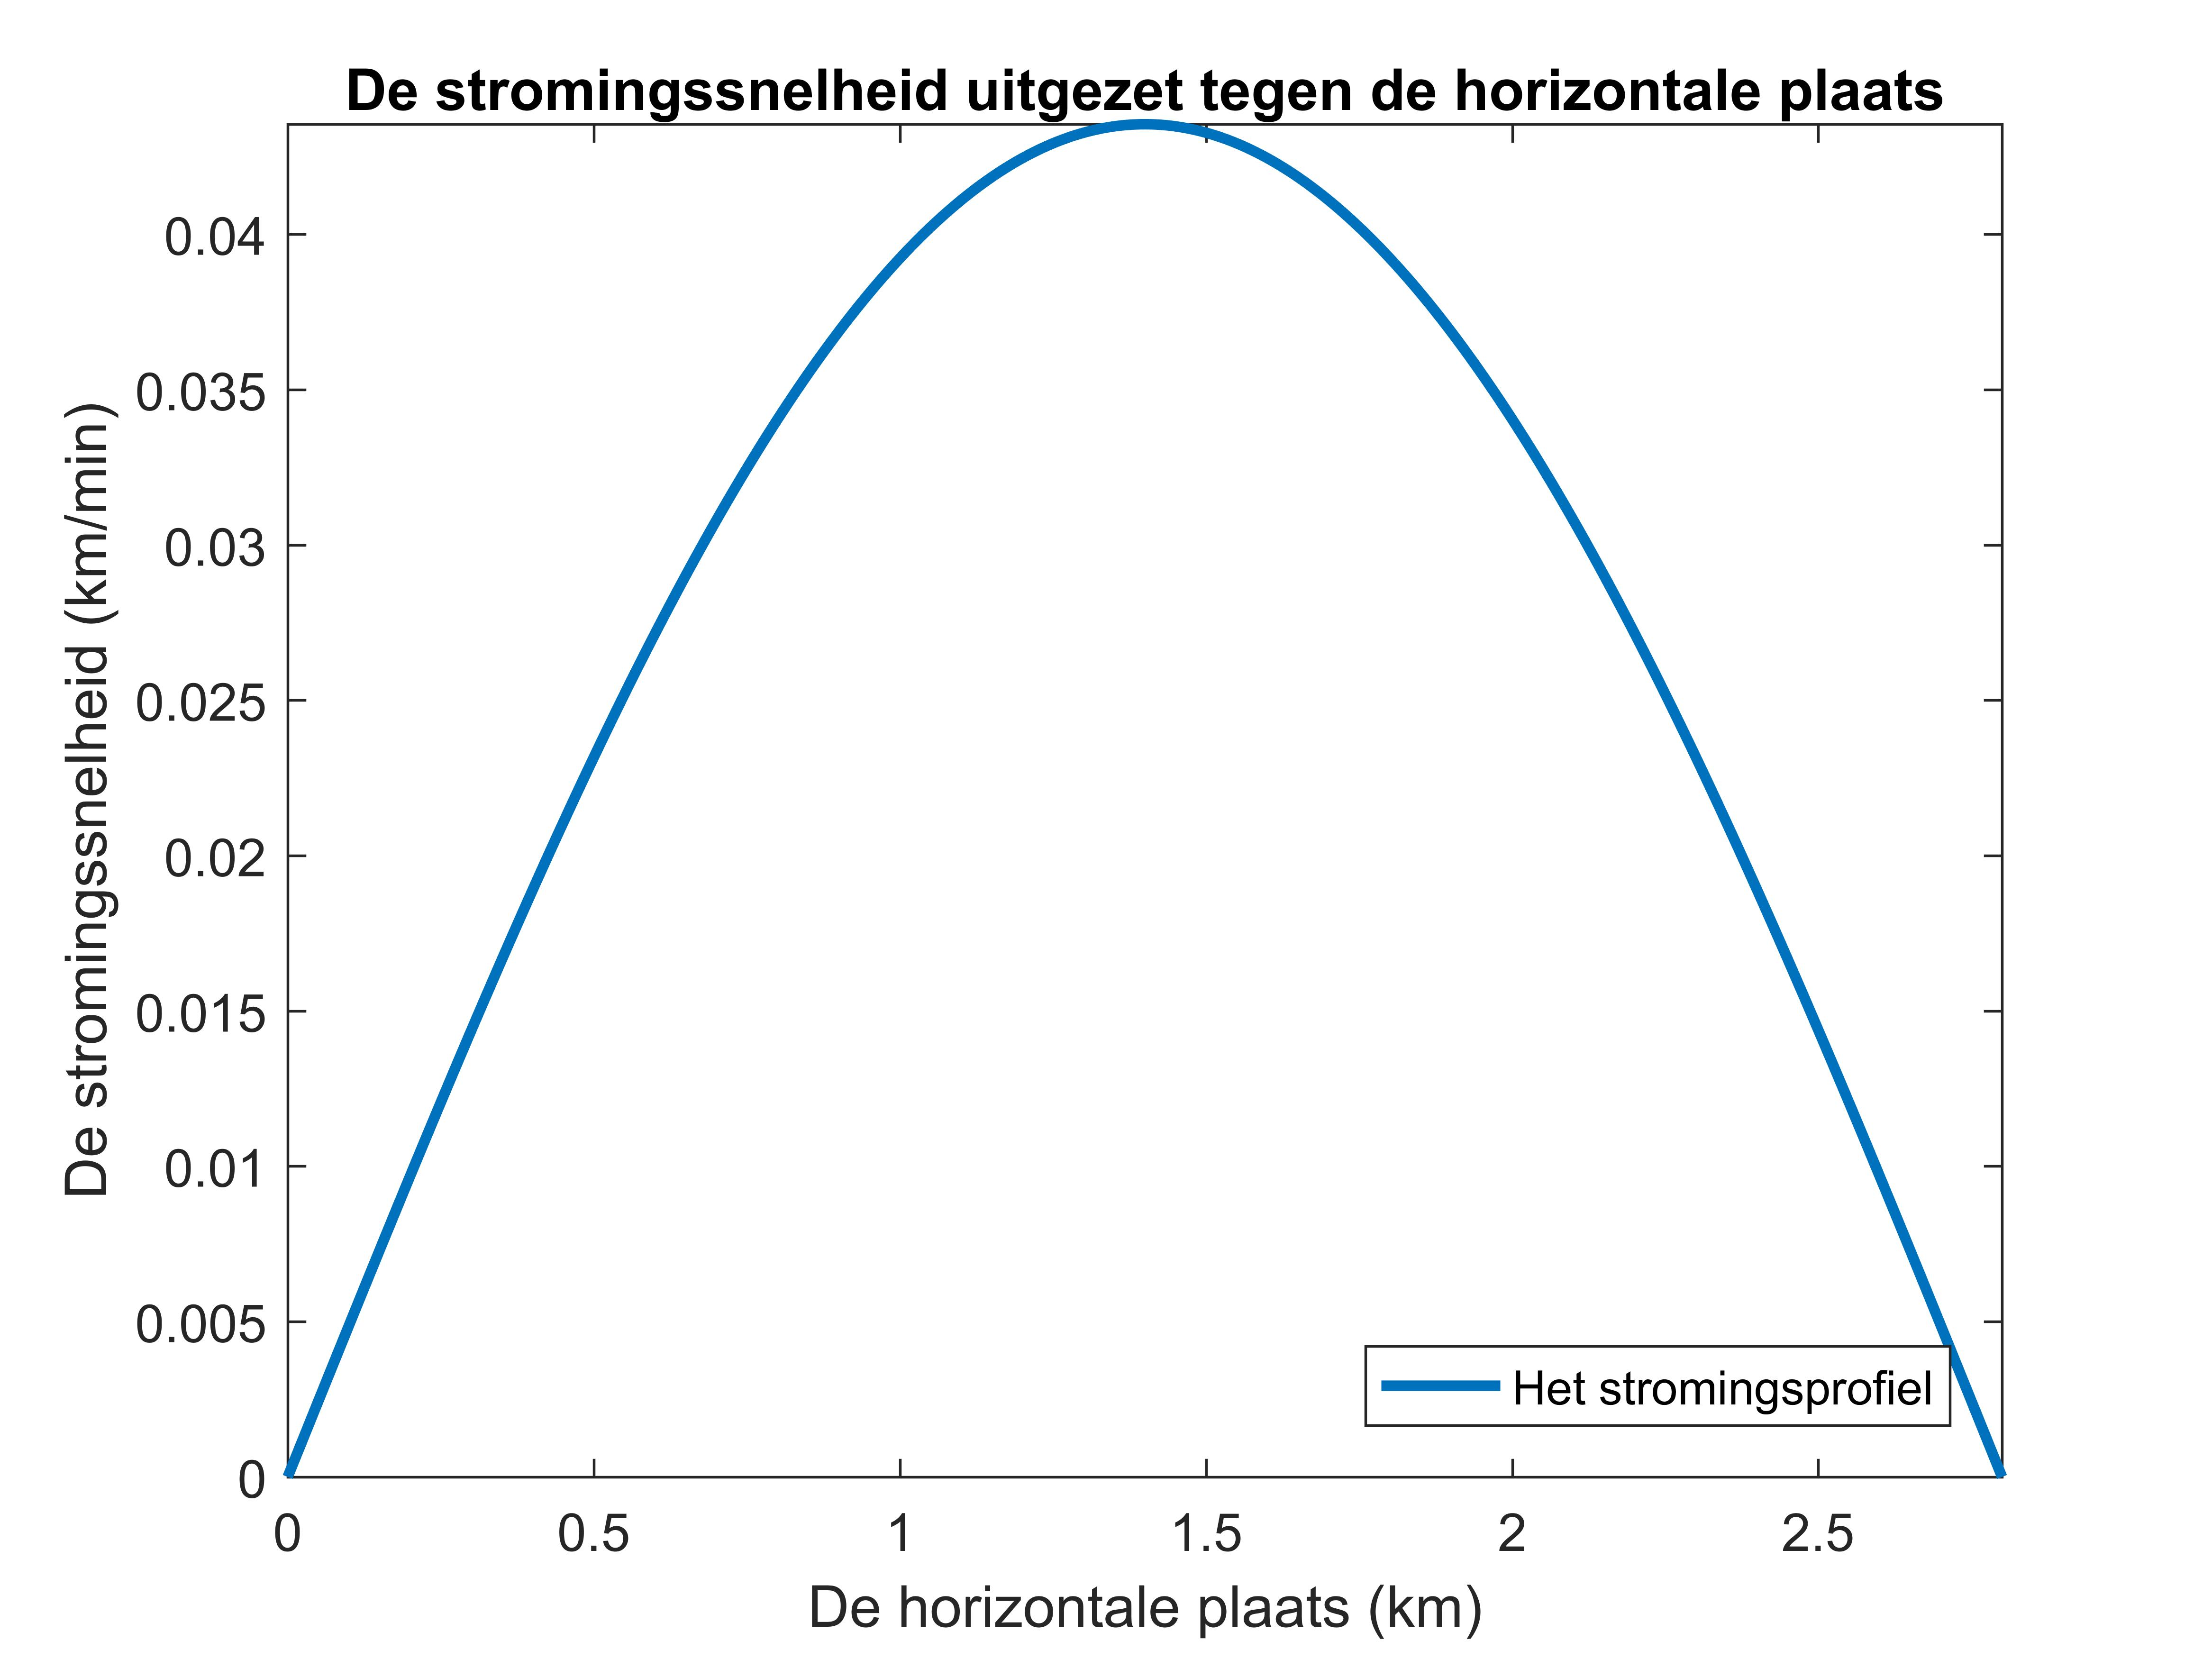
\includegraphics[width=\linewidth]{Sin_stroming_4.jpg}\label{fig:sinstroom}
	\caption{Een mogelijk stromingsprofiel voor de Nijl}
\end{figure}

Door de eerdere eisen in te vullen in MATLAB vinden we voor een boot met een snelheid van \(1~km/min\) een eindtijd van \(T=2.87\) minuten. De resultaten zijn in onderstaande figuren weergegeven.\\
\begin{figure}[H]
	\centering
	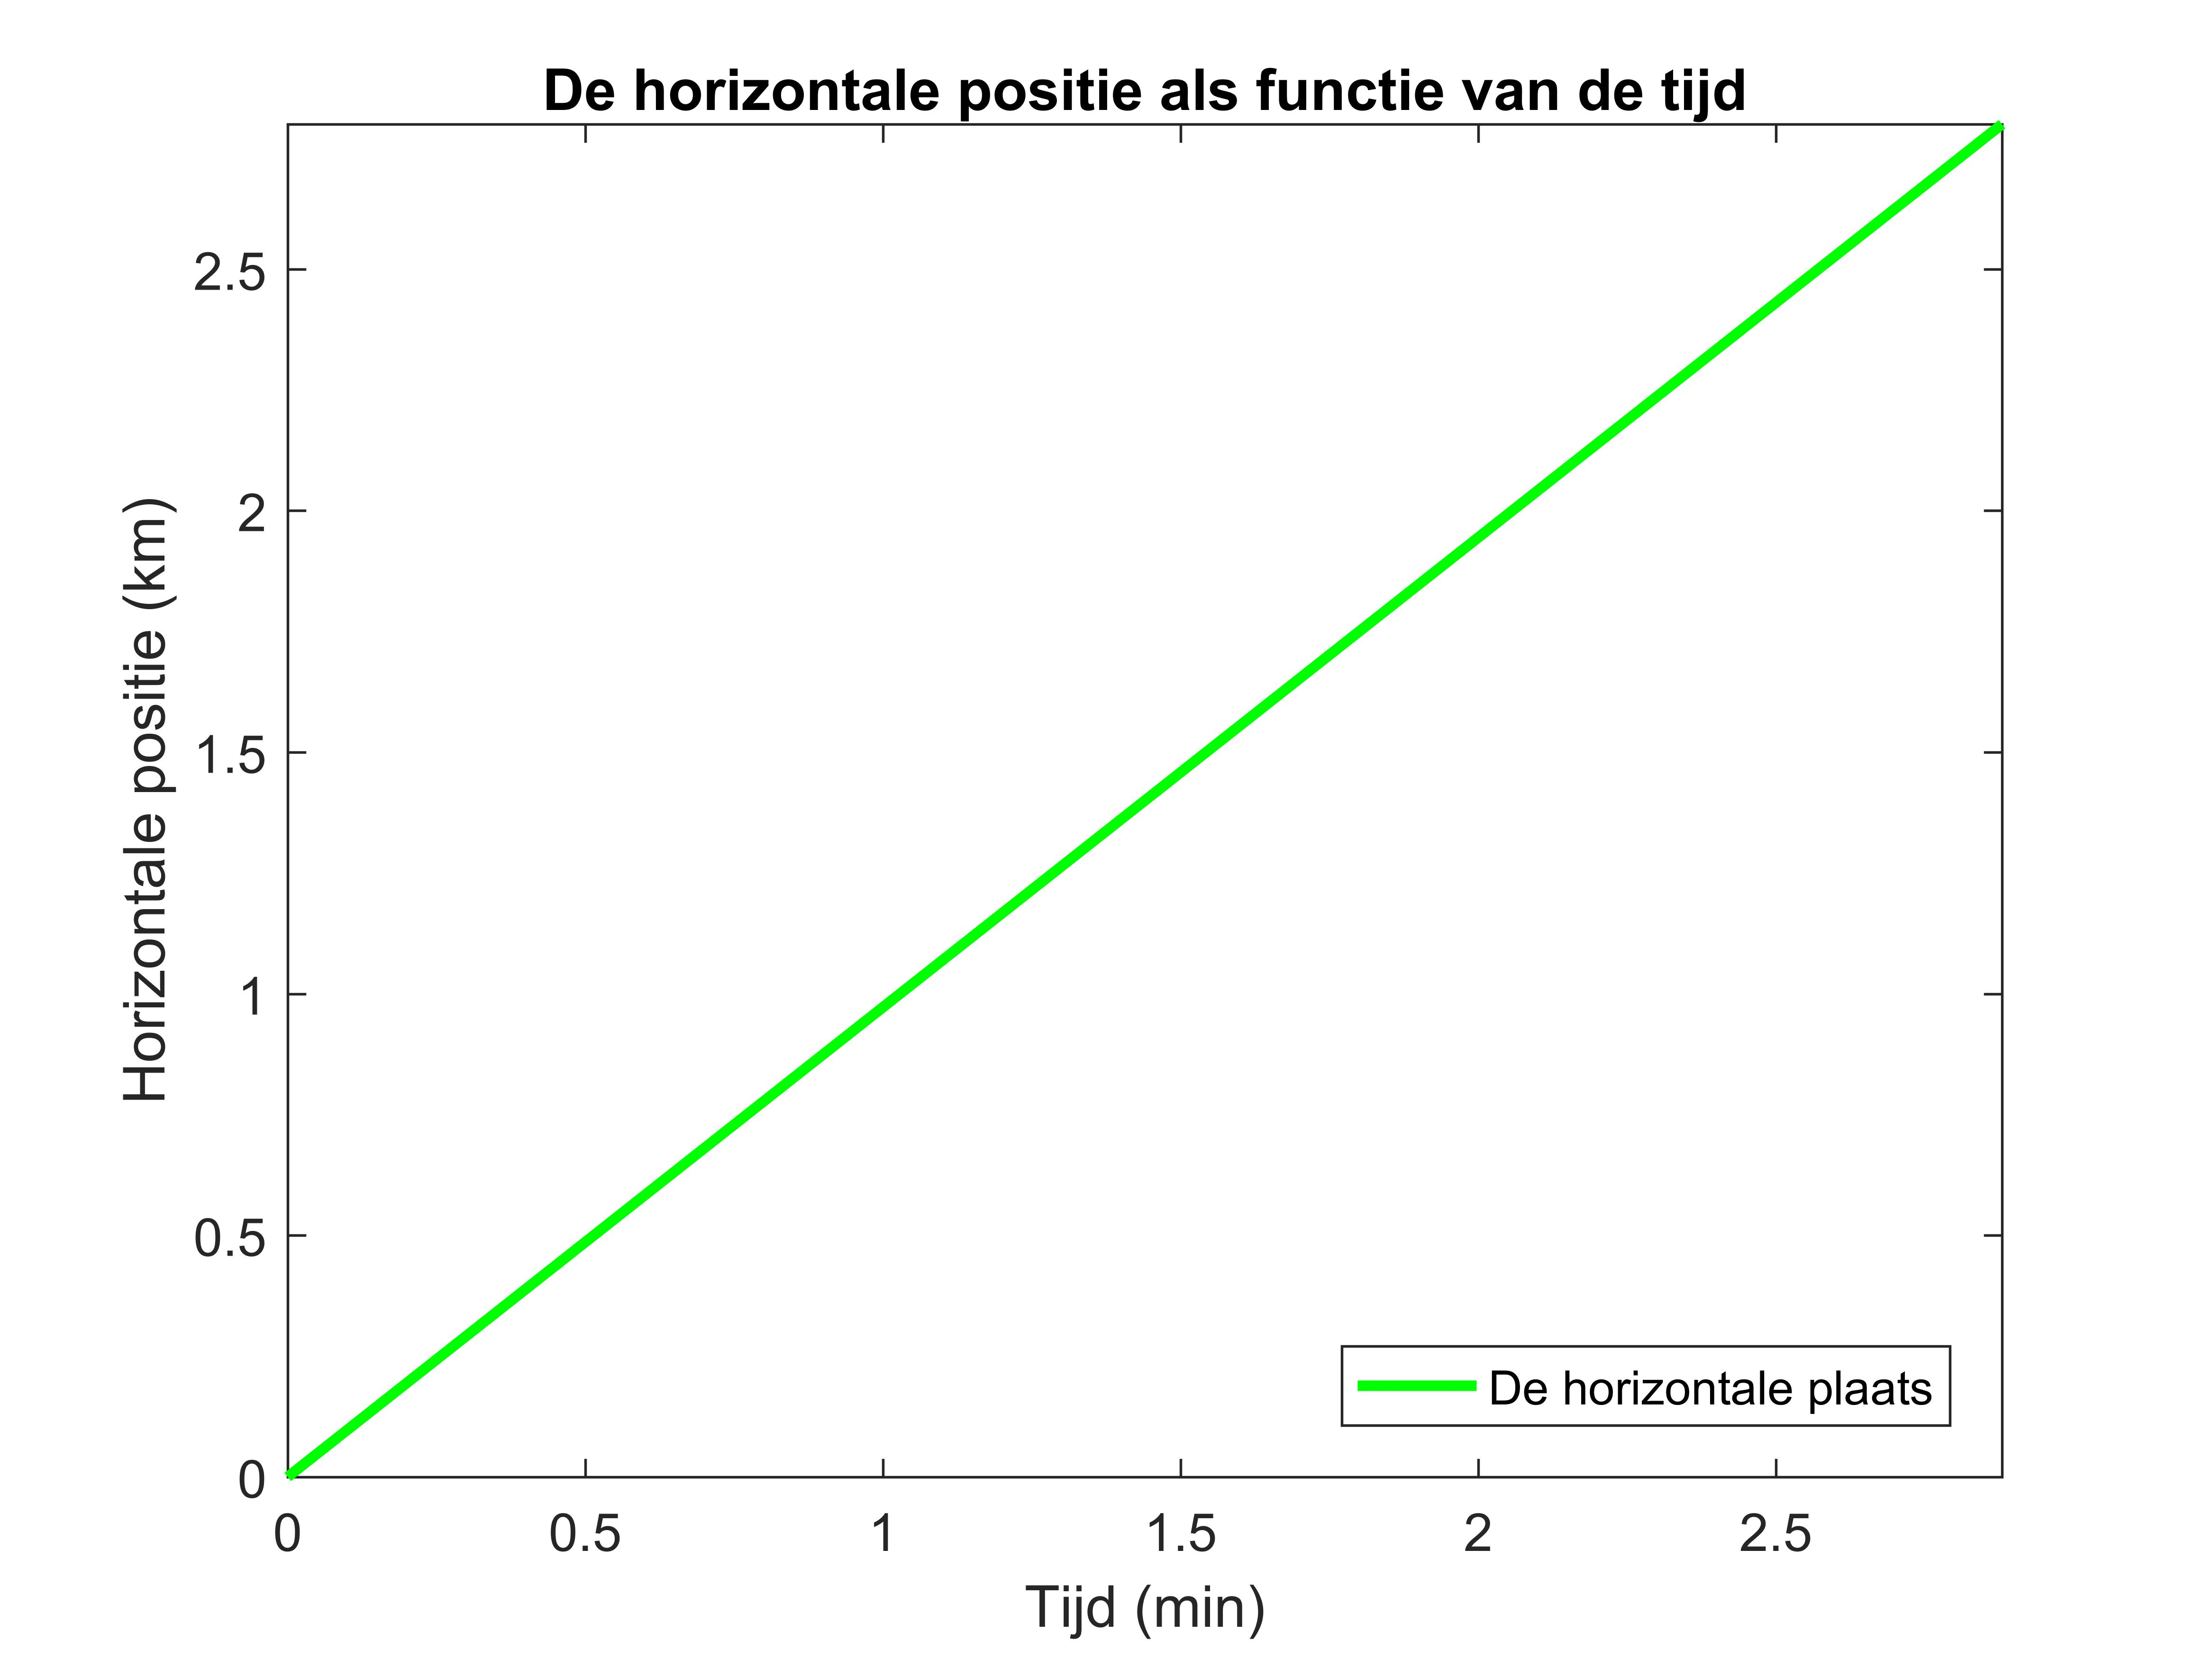
\includegraphics[width=\textwidth]{Sin_xt_3.jpg}
	\caption{De horizontaal positie \(x_1\) uitgezet tegen de tijd \(t\) tijdens een oversteek van de Nijl}\label{fig:sinplots1}
\end{figure}
Figuur \ref{fig:sinplots1} geeft het verband aan tussen de horizontale plaats (de afgelegde afstand ten opzicht van de oever) en de tijd van aankomst bij een punt.
Dit verband is lineair de snelheid in de horizontale richting is dus constant (\(v=\frac{dx_1}{dt}=c\)). \(T=2.87\) en \(x_1(T)=2.8\).
De horizontale snelheid is dus kleiner dan de totale snelheid van de boot.

\begin{figure}[H]
	\centering
	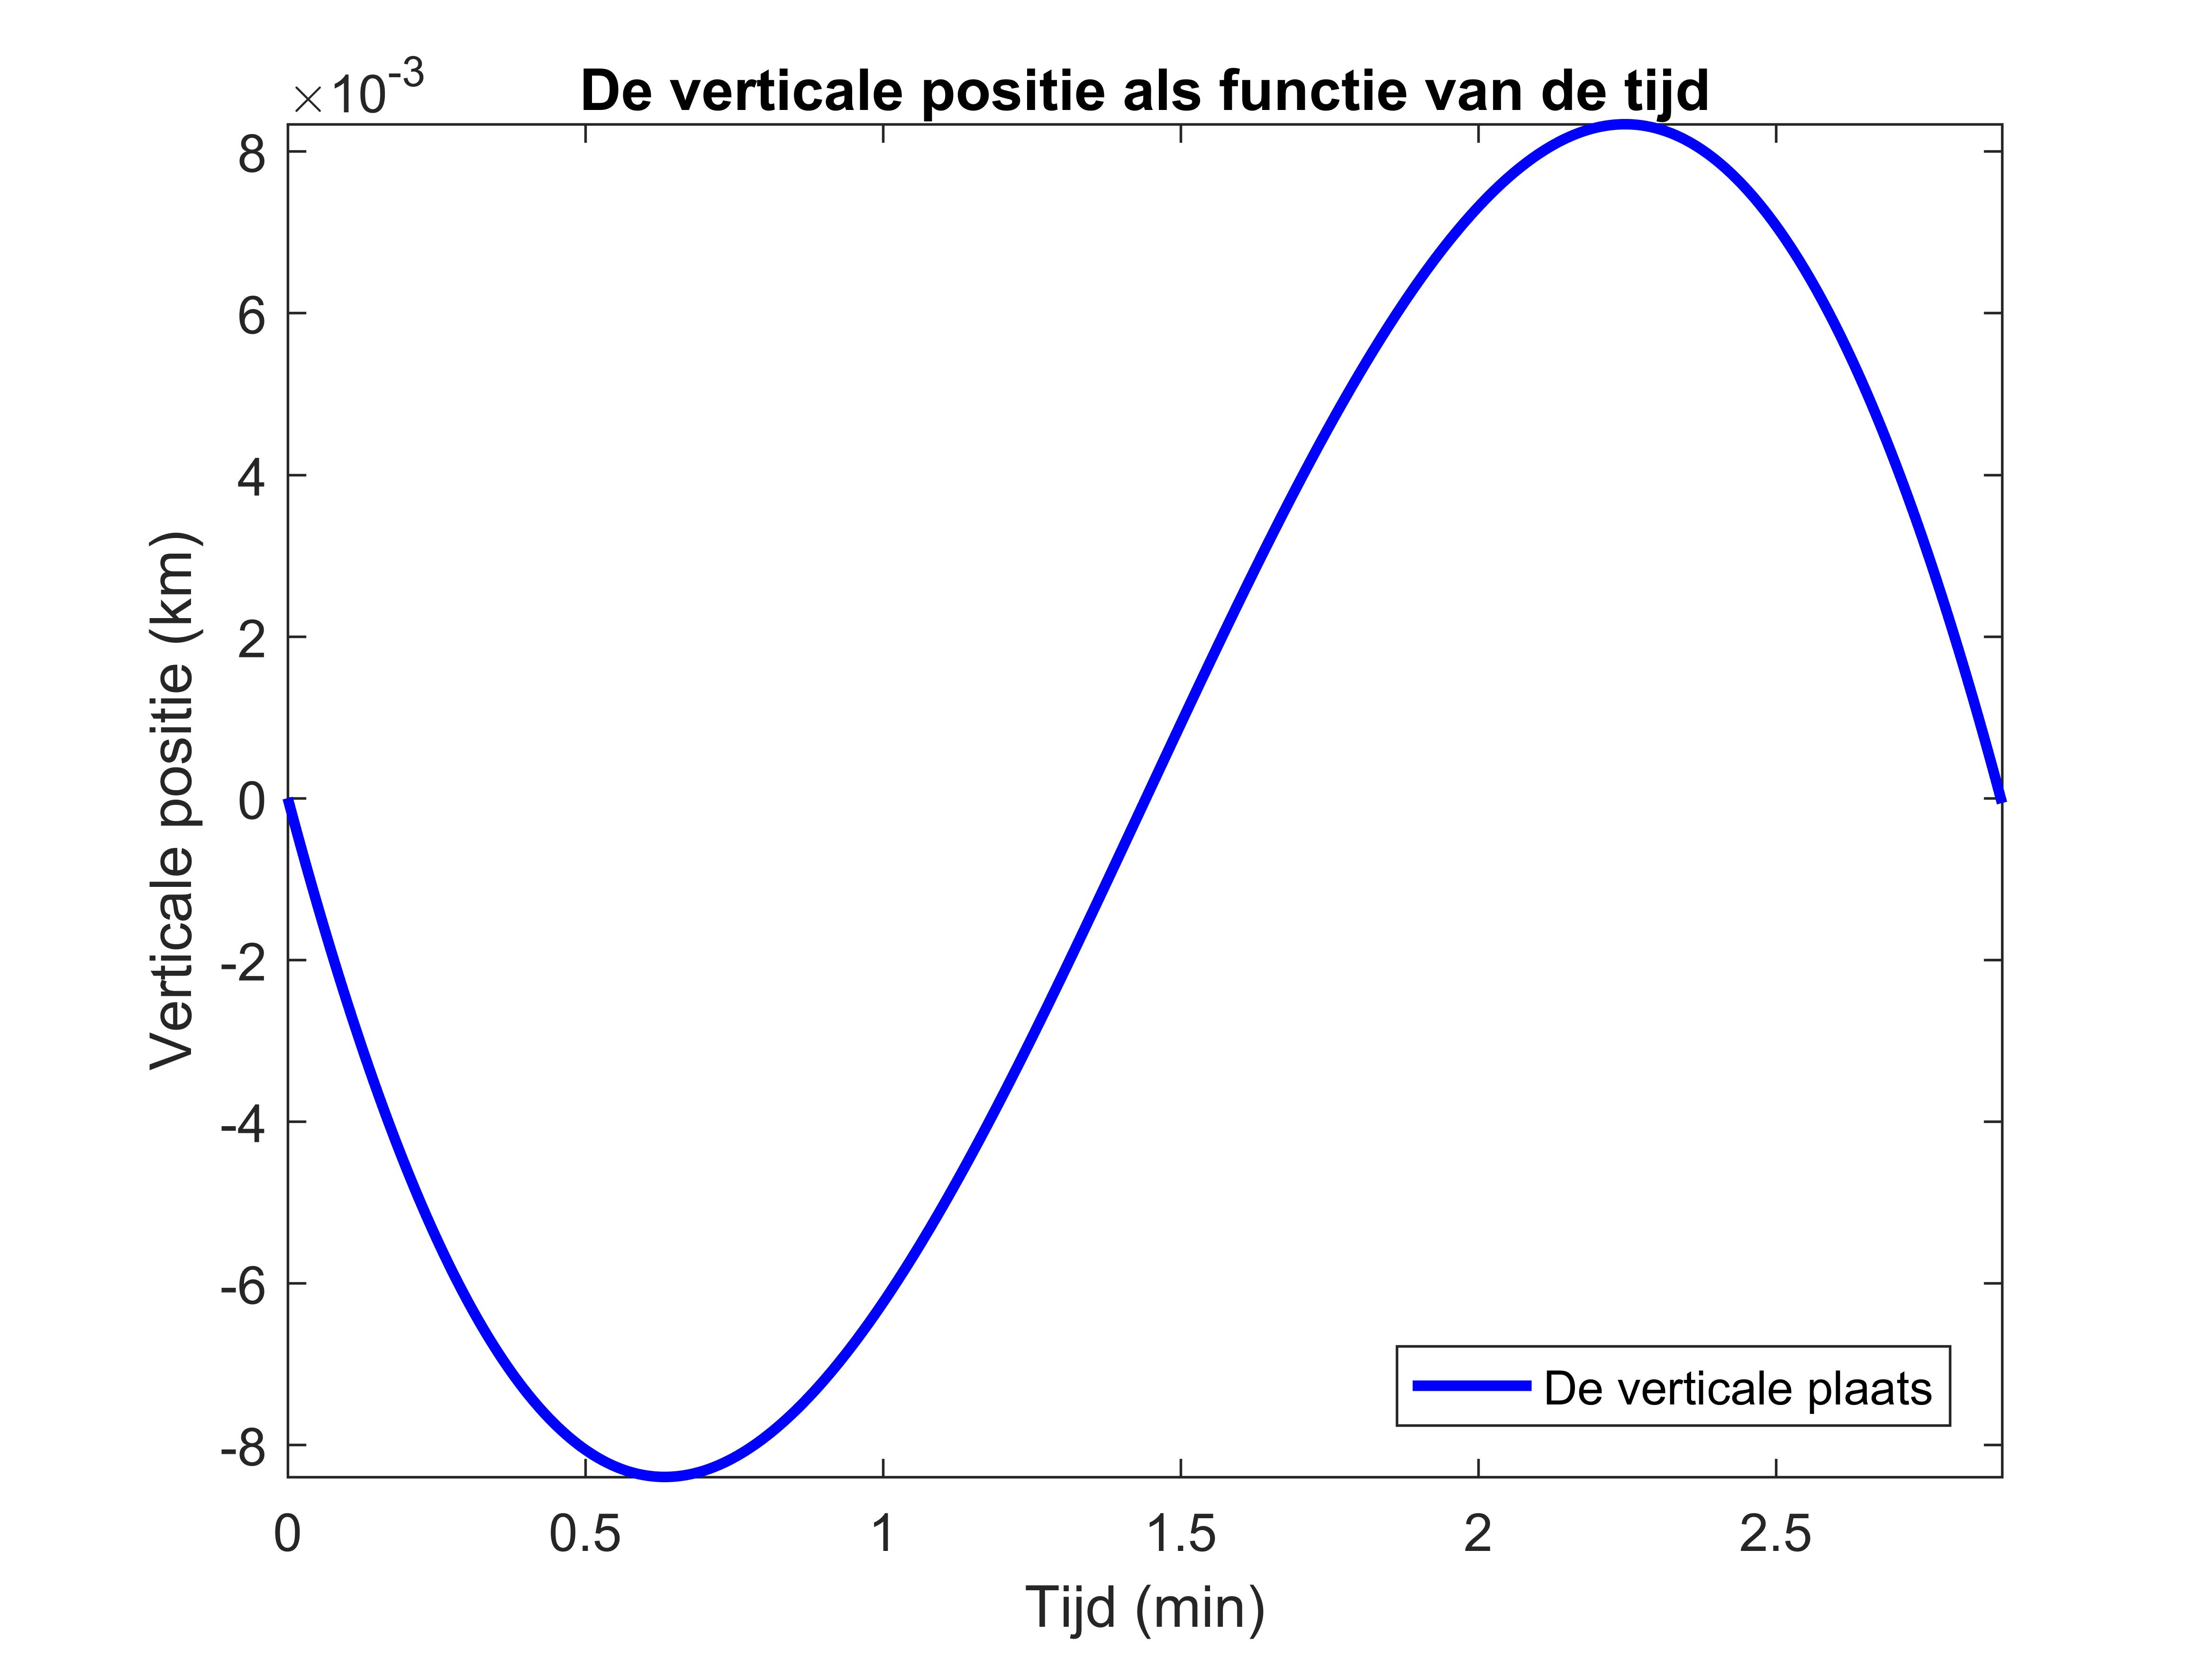
\includegraphics[width=\textwidth]{Sin_yt_2.jpg}
	\caption{De verticale positie \(x_2\) uitgezet tegen de tijd \(t\) tijdens een oversteek van de Nijl}\label{fig:sinplots2}
\end{figure}
Figuur \ref{fig:sinplots2} geeft de verticale plaats aan op een tijdstip \(t\).
Dit verband wordt beschreven door een sinuso\"ide.
De oorzaak hiervan wordt beschreven bij figuur \ref{fig:sinplots3}.
Het is hierbij opmerkelijk dat de verticale positie een hele lage amplitude heeft.
De verticale positie heeft een orde van grootte van \(10^{-3}~km\).
De boot zal tijdens een pad hoogstens 8 meter verwijderd zijn van zijn startpunt (verticaal gezien).

\begin{figure}[H]
	\centering
	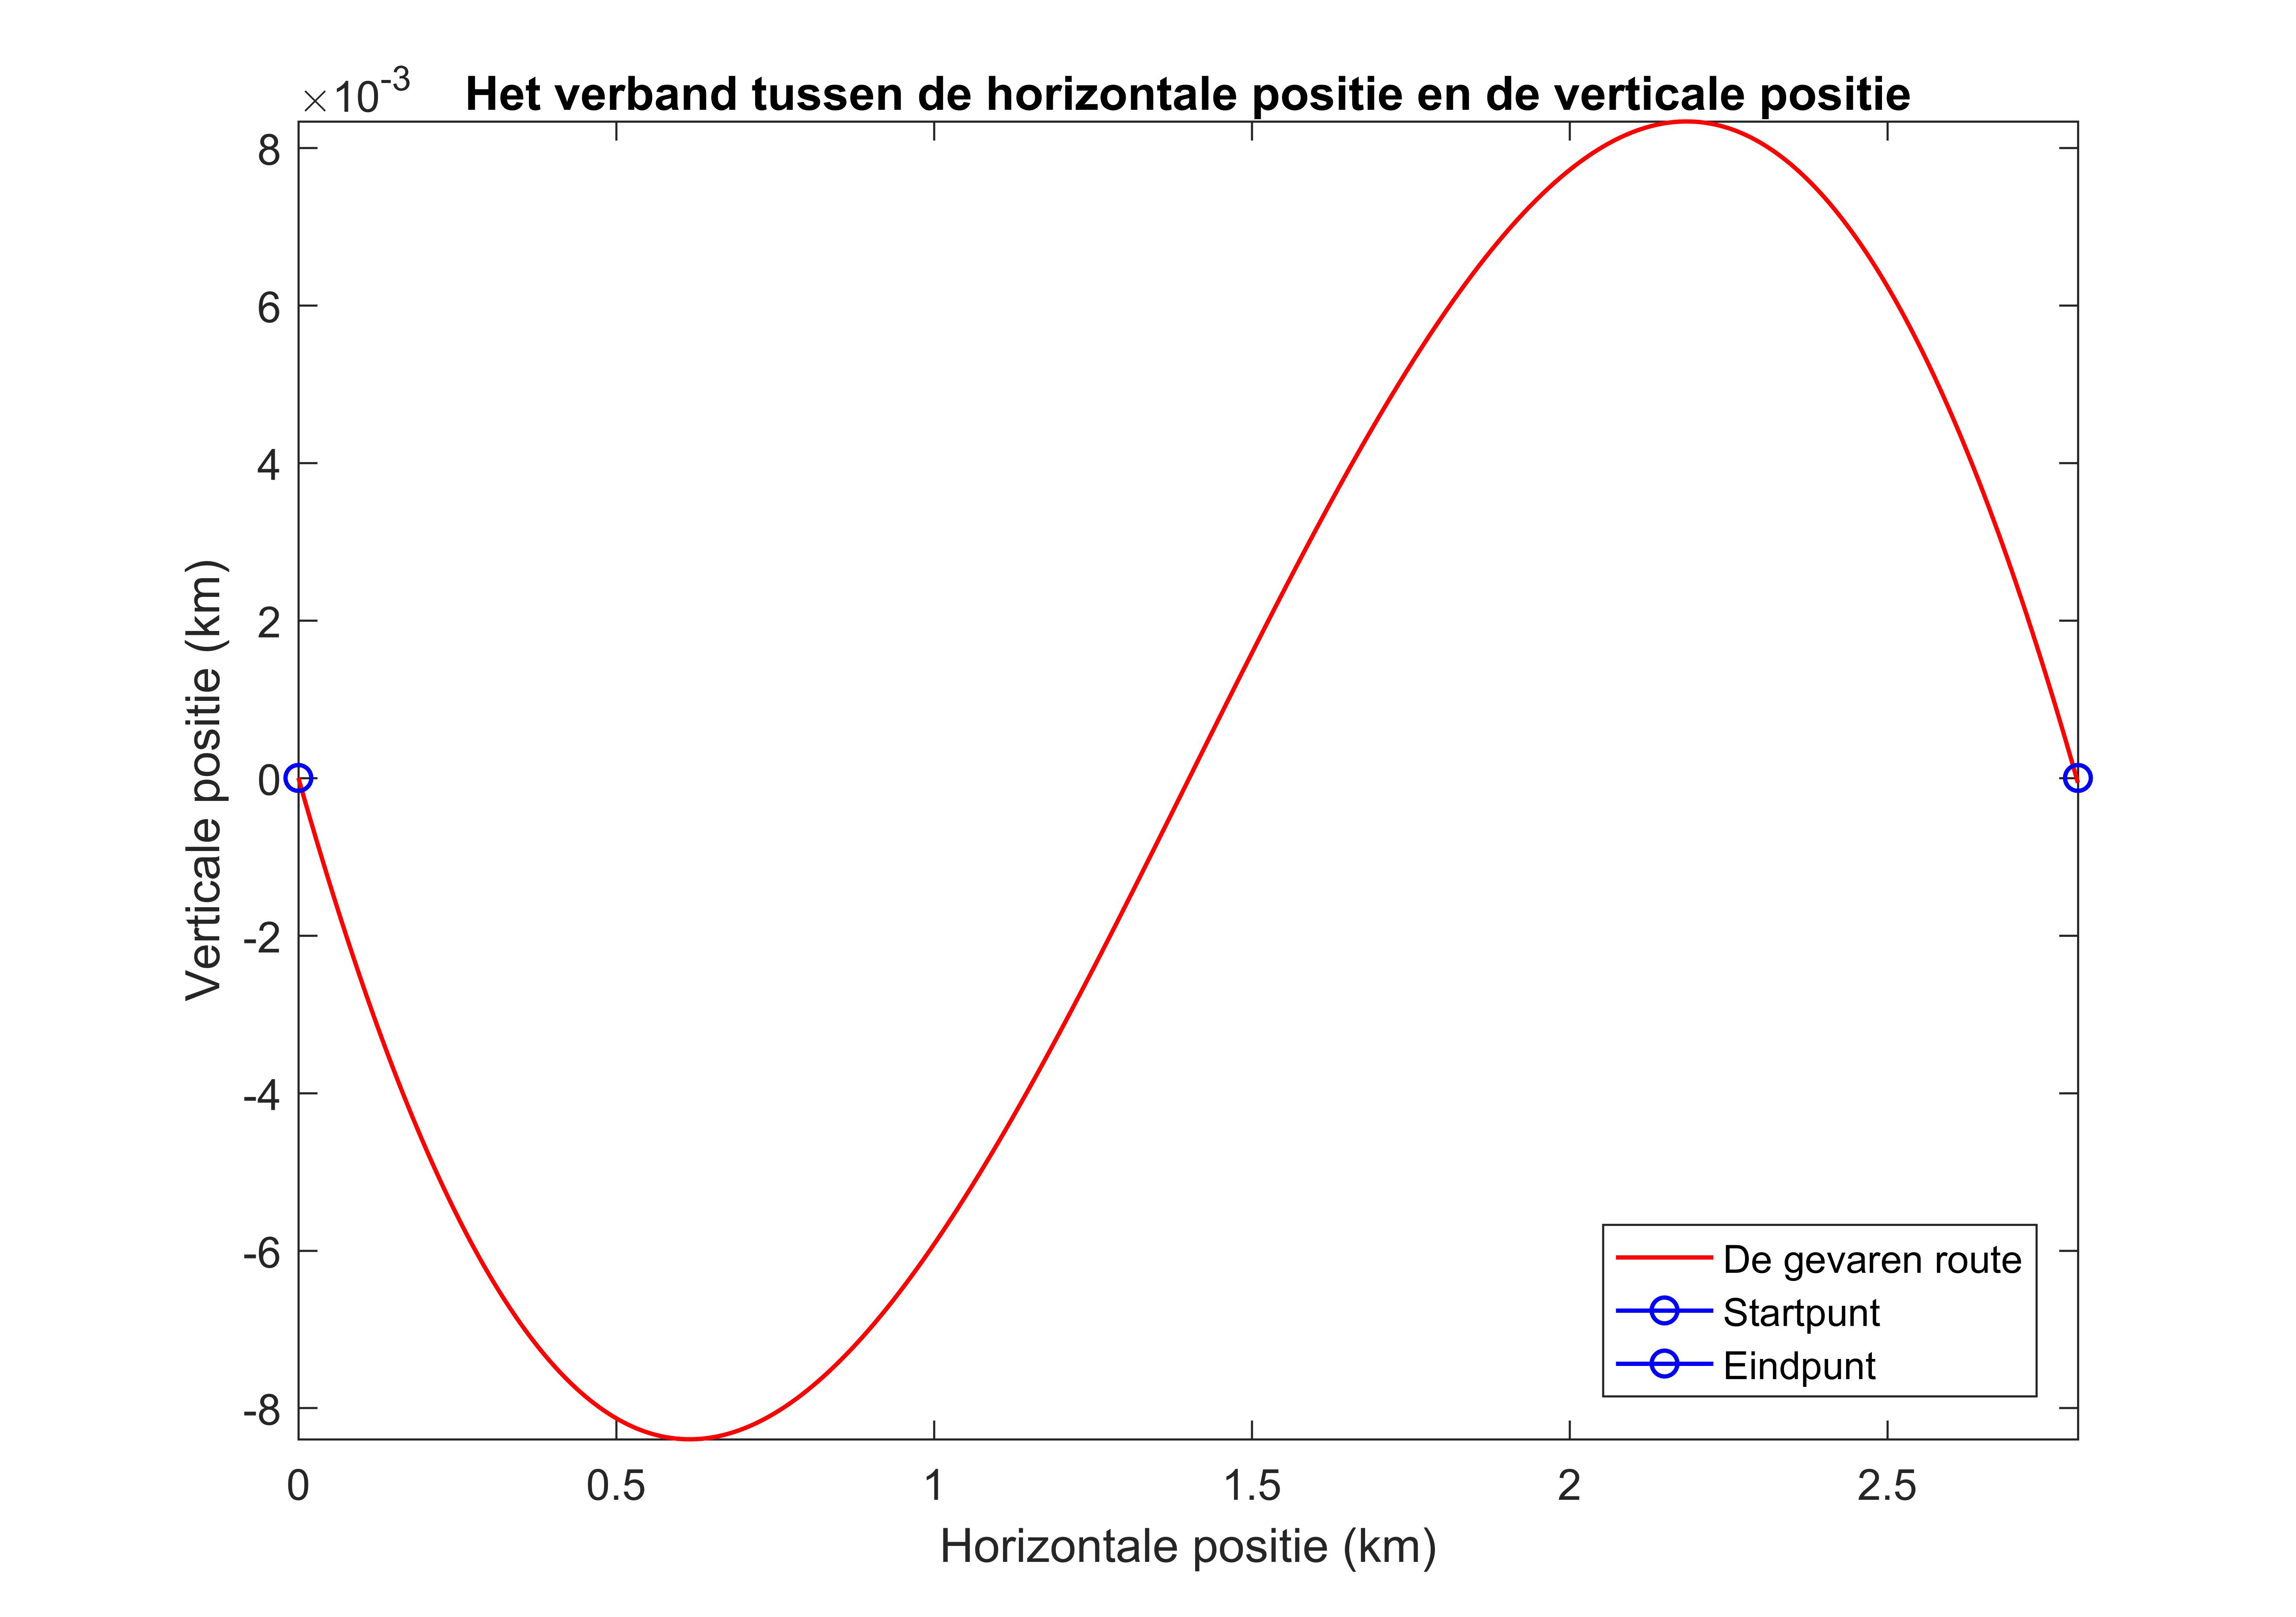
\includegraphics[width=\textwidth]{Sin_xy_2.jpg}
	\caption{Het afgelegde pad tijdens een oversteek van de Nijl}\label{fig:sinplots3}
\end{figure}
Figuur \ref{fig:sinplots3} beschrijft het verloop van een oversteek.
Voor elk tijdstip \(t\) wordt \(x_2(t)\) uitgezet tegen \(x_1(t)\).
Deze vorm beschrijft bijna exact dezelfde sinuso\"ide als de sinuso\"ide gegeven in figuur \ref{fig:sinplots2}.
Dit komt omdat \(x_1(t)\) lineair is ten opzichte van \(t\) en zelfs bijna evenredig: \(x_1(t)= \frac{x_1(T)}{T}t=\frac{2.8}{2.87}t\approx 0.97t\).
De sinuso\"ide vorm kan verklaard worden aan de hand van de stromingsfunctie \(S(x_1)\).
De stroming is zwak aan de oevers en sterk in het midden van de rivier.
Als we dus bij de oevers sterk tegen de stroming invaren, kunnen we in het midden van de rivier deze uitwijking gebruiken als extra versnelling (of minder vertraging).
De daar opgelopen uitwijking stroomafwaarts kan dan weer worden bijgestuurd als de stroming zwak is.
\begin{figure}[H]
	\centering
	\includegraphics[width=\textwidth]{Sin_stuur_4.jpg}
	\caption{De stuurhoek uitgezet tegen de tijd tijdens een oversteek van de Nijl}\label{fig:sinplots4}
\end{figure}
Tot slot wordt in figuur \ref{fig:sinplots4} de stuurhoek uitgezet tegen de tijd.
De stuurhoek is overal negatief, en het sterkst negatief in het midden van de rivier.
Als de stroming het sterkst is, draait de boot dus sterk bij om zijn richting voldoende bij te draaien, zodat hij met een maximale snelheid richting het eindpunt kan varen als de stroming zwakker is.\\

Deze plots zijn allemaal bepaald voor een boot met een snelheid van \(1~km/min\).
Onze boot heeft echter geen snelheid van \(1~km/min\) maar \(0.63~km/min\) Onze boot zal er dus in totaal \(\frac{T}{0.63}=4.57\)minuten over doen.
